\section{Desarrollo}



\begin{section-theorem.tcb}{Teorema de Pascal}{pascal-theorem}
    Sea $ABCDEF$ un héxagono inscrito (no necesariamente convexo) en una círcunferencia $\Omega$.
    Entonces, los puntos $M = AB \cap DE$, $N = BC \cap EF$ y $P = CD \cap FA$ son colineales.
\end{section-theorem.tcb}

\begin{proof}
    Sean $X = BC \cap DE$, $Y = DE \cap FA$ y $Z = FA \cap BC$.

    \begin{multicols}{2}
        \begin{figure}[H]
            \centering
            \begin{tikzpicture}[xscale = 1.5, yscale = 1.5]

\end{tikzpicture}
        \end{figure}
        Al usar el teorema de \textbf{Menelao} tres veces en \theTriangle{XYZ}, primero con la transversal $A - B - M$, después con la transversal $P - C - D$ y finalmente con $F - N - E$, respectivamente, obtenemos que
        \begin{align*}
            &\rations{Z}{X}{Y}{M}{A}{B} = 1,\\[3mm]
            &\rations{Z}{X}{Y}{D}{P}{C} = 1\ \text{y}\\[3mm]
            &\rations{Z}{X}{Y}{E}{F}{N} = 1.
        \end{align*}
    \end{multicols}
    \vspace{-10mm}
    Multiplicando estas tres igualdades y reordenando los miembros, obtenemos que
    \begin{align*}
        \frac{XM}{MY} \cdot \frac{XM}{MY} \cdot \frac{XM}{MY} \cdot \frac{(YA\cdot YF) \cdot (ZB\cdot ZC) \cdot (XD\cdot XE)}{(AZ\cdot FZ) \cdot (BX \cdot CX) \cdot (DY\cdot EF)} = 1. \tag{$\ast$}
    \end{align*}
    Ahora por la \textbf{Propiedad~\ref{power-external-point}} sabemos que para los puntos $X$, $Y$ y $Z$ se cumple que
    \begin{align*}
        XD \cdot XE = XC \cdot XB \quad \land \quad
        YF \cdot YA = YE \cdot YD \quad \land \quad
        ZB \cdot ZC = ZA \cdot ZE
    \end{align*}
    Así $(\ast)$ se convierte en
    \[
        \rations{Z}{X}{Y}{M}{P}{N} = 1,
    \]
    que por el teorema de \textbf{Menelao} significa que $M$, $N$ y $P$ son colineales.
\end{proof}

\begin{remark.tcb}
    Una manera fácil de recordar las intersecciones es la siguiente:
    Tomamos dos letras consecutivas, dejamos una letra de espacio, y tomamos otras dos letras consecutivas.
    La intersección de las rectas formadas con eso pares puntos es el primer punto de la colinealidad.
    Luego nos movemos a la derecha y repetimos el proceso dos veces más.\footnote{Otra manera de verlos es tomar vértices consecutivos módulo 3.}
    \begin{multicols}{2}
        \begin{figure}[H]
            \centering
            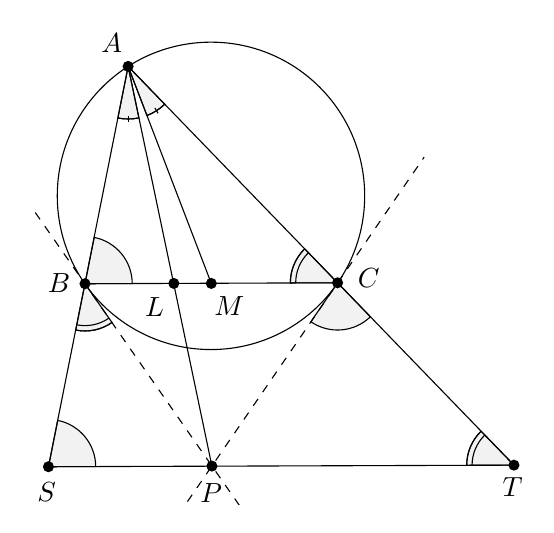
\begin{tikzpicture}[scale = 0.4]
    \clip(-2.36,-10.08) rectangle (13.47,5.06);
    \draw [shift={(-0.54,-3.07)},fill=black,fill opacity=0.05] (0,0) -- (0.2:1.5) arc (0.2:78.71:1.5) -- cycle;
    \draw [shift={(7.48,-3.04)},fill=black,fill opacity=0.05] (0,0) -- (-124.46:1.5) arc (-124.46:-45.95:1.5) -- cycle;
    \draw [shift={(-1.7,-8.88)},fill=black,fill opacity=0.05] (0,0) -- (0.2:1.5) arc (0.2:78.71:1.5) -- cycle;
    \draw [shift={(-0.54,-3.07)},fill=black,fill opacity=0.05] (0,0) -- (-101.29:1.5) arc (-101.29:-55.14:1.5) -- cycle;
    \draw [shift={(7.48,-3.04)},fill=black,fill opacity=0.05] (0,0) -- (134.05:1.5) arc (134.05:180.2:1.5) -- cycle;
    \draw [shift={(13.08,-8.83)},fill=black,fill opacity=0.05] (0,0) -- (134.05:1.5) arc (134.05:180.2:1.5) -- cycle;
    \draw [shift={(0.83,3.83)},fill=black,fill opacity=0.05] (0,0) -- (-101.29:1.67) arc (-101.29:-78.18:1.67) -- cycle;
    \draw [shift={(0.83,3.83)},fill=black,fill opacity=0.05] (0,0) -- (-69.06:1.67) arc (-69.06:-45.95:1.67) -- cycle;
    \draw(3.46,-0.28) circle (4.88cm);
    \draw (-0.54,-3.07)-- (7.48,-3.04);
    \draw (0.83,3.83)-- (-1.7,-8.88);
    \draw (0.83,3.83)-- (13.08,-8.83);
    \draw (-1.7,-8.88)-- (13.08,-8.83);
    \draw (0.83,3.83)-- (3.49,-8.86);
    \draw (0.83,3.83)-- (3.47,-3.06);
    \draw [dash pattern=on 3pt off 3pt,domain=-2.1176316762214267:13.472829432059696] plot(\x,{(-21.59-8.05*\x)/5.61});
    \draw [dash pattern=on 3pt off 3pt,domain=-2.361745286484902:10.226227746616733] plot(\x,{(--93.93-9.81*\x)/-6.74});
    \draw [shift={(-0.54,-3.07)}] (-101.29:1.5) arc (-101.29:-55.14:1.5);
    \draw [shift={(-0.54,-3.07)}] (-101.29:1.33) arc (-101.29:-55.14:1.33);
    \draw [shift={(7.48,-3.04)}] (134.05:1.5) arc (134.05:180.2:1.5);
    \draw [shift={(7.48,-3.04)}] (134.05:1.33) arc (134.05:180.2:1.33);
    \draw [shift={(13.08,-8.83)}] (134.05:1.5) arc (134.05:180.2:1.5);
    \draw [shift={(13.08,-8.83)}] (134.05:1.33) arc (134.05:180.2:1.33);
    \draw [shift={(0.83,3.83)}] (-101.29:1.67) arc (-101.29:-78.18:1.67);
    \draw(0.84,2.27) -- (0.84,2.07);
    \draw [shift={(0.83,3.83)}] (-69.06:1.67) arc (-69.06:-45.95:1.67);
    \draw(1.68,2.51) -- (1.78,2.34);
    \begin{scriptsize}
        \normalsize
        \fill [color=black] (0.83,3.83) circle (5pt);
        \draw[color=black] (0.31,4.56) node {$A$};
        \fill [color=black] (3.49,-8.86) circle (5pt);
        \draw[color=black] (3.47,-9.7) node {$P$};
        \fill [color=black] (-0.54,-3.07) circle (5pt);
        \draw[color=black] (-1.36,-3.04) node {$B$};
        \fill [color=black] (7.48,-3.04) circle (5pt);
        \draw[color=black] (8.47,-2.88) node {$C$};
        \fill [color=black] (-1.7,-8.88) circle (5pt);
        \draw[color=black] (-1.76,-9.68) node {$S$};
        \fill [color=black] (13.08,-8.83) circle (5pt);
        \draw[color=black] (13.04,-9.54) node {$T$};
        \fill [color=black] (2.28,-3.06) circle (5pt);
        \draw[color=black] (1.67,-3.81) node {$L$};
        \fill [color=black] (3.47,-3.06) circle (5pt);
        \draw[color=black] (4.04,-3.78) node {$M$};
    \end{scriptsize}
\end{tikzpicture}
            \caption{Teorema de Pascal.}
            \label{fig:pascal-theorem}
        \end{figure}
        \hfill\\
        \hfill\\
        \hfill\\
        \hfill
        \begin{figure}[H]
            \centering
            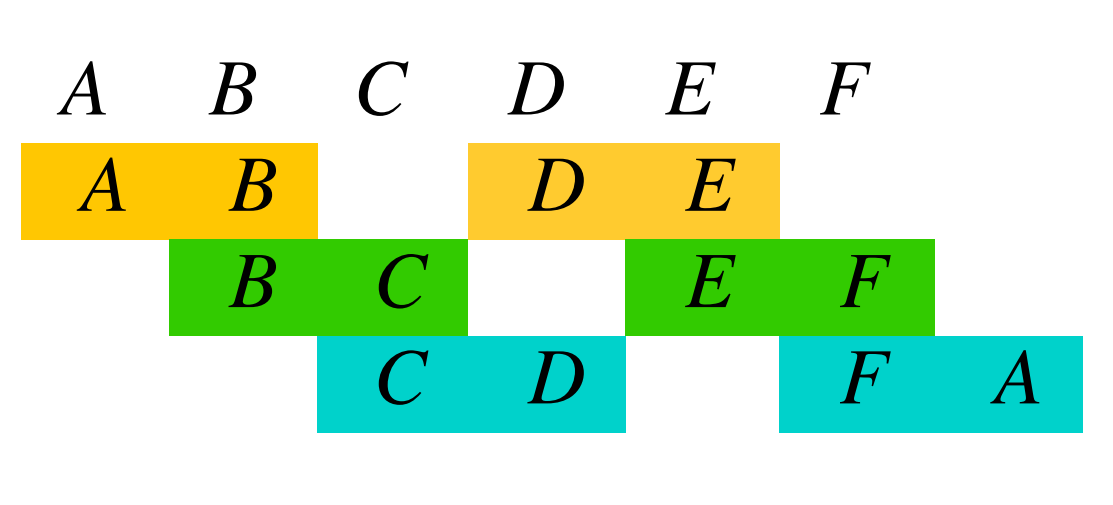
\includegraphics[width=0.4\textwidth]{images/pascal-mnemotec}
            \caption{Mnemotécnia de Pascal.}
        \end{figure}
    \end{multicols}
\end{remark.tcb}


El~\refTheorem{\ref{t:pascal-theorem}} es independiente de cómo haya sido tomado el hexágono.
El mostrado en la demostración es el caso más sencillo en el cual el hexágono es convexo.
Sin embargo, la colinealidad se sigue cumpliendo aunque el hexágono no sea convexo, como se puede ver en la figura \ref{fig:pascal-theorem}.
La demostración de este caso y de cualquier otro es análoga a la primera.

\begin{section-example.tcb}{}{}
    Sean $D$ y $E$ los puntos medios de los arcos menores $\wideparen{AB}$ y $\wideparen{AC}$ del circuncírculo del \theTriangle{ABC}, respectivamente.
    Sea $P$ un punto en el arco menor $BC$, $Q = PD \cap AB$ y $R = PE \cap AC$.
    Probar que la recta $QR$ pasa a traves de incentro $I$ del \theTriangle{ABC}.
\end{section-example.tcb}

\begin{solution}
    Dado que $D$ es el punto medio del arco $\wideparen{AB}$, $CD$ es bisectriz del ángulo $\angle BCA$.
    Análogamentes, $BE$ es bisectriz de $\angle ABC$.
    Por lo tanto, $CD \cap BE = I$.
    Ahora, aplicando el~\refTheorem{\ref{t:pascal-theorem}} al hexágono $CDPEBA$ tenemos que los puntos $CD \cap BE = I$, $DP \cap BA = Q$ y $PE \cap AC = R$ son colineales.
\end{solution}


El~\refTheorem{\ref{t:pascal-theorem}} puede presentar versiones degeneradas, aunque puede suceder, el caso más habitual ya no consiste en un paralelismo, sino en la transformación de un polígono de seis lados a un polígono de cinco, cuatro o tres lados.
Como lo podemos ver en el siguiente ejemplo.

\begin{section-example.tcb}{}{}
    Sea $\omega$ el circuncírculo del \theTriangle{ABC}.
    Las tangentes a $\omega$ por lo puntos $A$, $B$ y $C$ intersecan a las rectas $BC$, $CA$ y $AB$ en los puntos $D$, $E$ y $F$, respectivamente.
    Probar que los puntos $D$, $E$ y $F$ está alineados.
\end{section-example.tcb}

\begin{solution}
    Aplicando el~\refTheorem{\ref{t:pascal-theorem}} al hexágono $AABBCC$.
    Tenemos que los puntos $AA \cap BC = D$, $AB \cap CC = F$ y $BB \cap CA = E$ son colineales.
\end{solution}

\begin{remark.tcb}

\end{remark.tcb}



\newpage
\begin{section-theorem.tcb}{Teorema de Brianchon}{brianchon-theorem}
    Sea $ABCDEF$ un hexágono circunscrito (no necesariamente convexo) a un círculo $\Omega$.
    Entonces, las rectas $AD$, $BE$ y $CF$ son concurrentes.
\end{section-theorem.tcb}




\subsection{Agregados culturales y preguntas}




\section{Conocimiento previo}

\begin{section-property}[Potencia de un punto exterior]\label{power-external-point}
Sean $AD$ y $CD$ dos rectas que se intersecan en $X$ tales que $X - A - B$ y $X - C - D$.
Entonces el cuadrilátero $ABCD$ es cíclico si y solo si
\[
    \overline{XA} \cdot \overline{XB} = \overline{XC} \cdot \overline{XD}.
\]\end{section-property}

\begin{multicols}{2}
    \begin{proof}
        Rápidamente nos damos cuenta de que $\angle CXB = \angle AXD\quad (\ast).$
        Entonces $ABCD$ es cíclico
        \begin{align*}
            &\iff \angle ABC = \angle ADC\\
            &\iff \angle XBC = \angle ADX\\
            &\overset{(\ast)}{\iff} \triangle XBC \sim \triangle XDA \ \overset{(\ast)}{\iff} \ \frac{\overline{XB}}{\overline{XC}} = \frac{\overline{XD}}{\overline{XA}}\\[2mm]
            &\iff \overline{XA} \cdot \overline{XB} = \overline{XC} \cdot \overline{XD}. \qedhere
        \end{align*}
    \end{proof}
    \begin{figure}[H]
        \centering
        \definecolor{ttttff}{rgb}{0.2,0.2,1}
%dash pattern=on 5pt off 2pt
%[fill = white, rounded corners = 4pt, inner sep = 1pt]
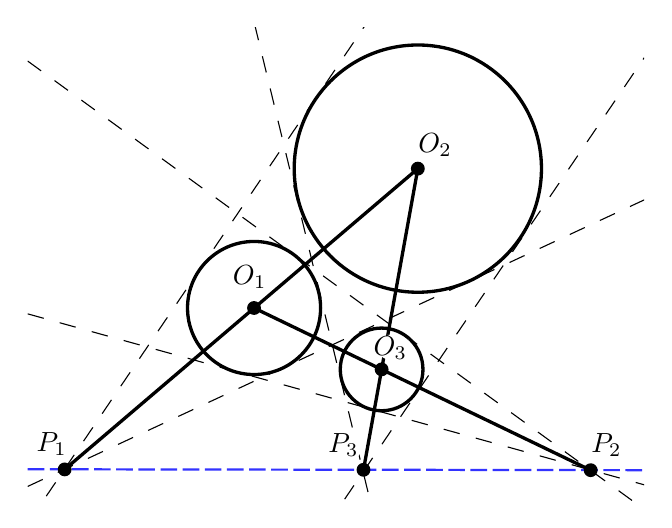
\begin{tikzpicture}[scale = 0.5]
    \clip(4.47,-5.82) rectangle (20.13,6.18);
    \draw [line width=1.2pt] (10.22,-0.94) circle (1.69cm);
    \draw [line width=1.2pt] (13.46,-2.5) circle (1.05cm);
    \draw [line width=1.2pt] (14.38,2.6) circle (3.14cm);
    \draw [line width=1.2pt] (5.41,-5.04)-- (14.38,2.6);
    \draw [line width=1.2pt] (14.38,2.6)-- (13,-5.05);
    \draw [line width=1.2pt] (10.22,-0.94)-- (18.77,-5.06);
    \draw [color = ttttff, dash pattern=on 6pt off 2pt, line width=0.8pt, domain=4.47:20.13] plot(\x,{(-67.19-0.02*\x)/13.36});
    \draw [dash pattern=on 6pt off 6pt,domain=4.47:20.13] plot(\x,{(-41.75--2.57*\x)/5.53});
    \draw [dash pattern=on 6pt off 6pt,domain=4.47:20.13] plot(\x,{(-44.52--5.05*\x)/3.42});
    \draw [dash pattern=on 6pt off 6pt,domain=4.47:20.13] plot(\x,{(-32.25--1.96*\x)/1.33});
    \draw [dash pattern=on 6pt off 6pt,domain=4.47:20.13] plot(\x,{(-27.15--2.31*\x)/-0.56});
    \draw [dash pattern=on 6pt off 6pt,domain=4.47:20.13] plot(\x,{(-40.25--3.41*\x)/-4.69});
    \draw [dash pattern=on 6pt off 6pt,domain=4.47:20.13] plot(\x,{(-0.84--1.55*\x)/-5.59});
    \begin{scriptsize}
        \normalsize
        \fill [color=black] (10.22,-0.94) circle (5pt);
        \draw[color=black] (10.11,-0.15) node[fill = white, rounded corners = 4pt, inner sep = 1pt] {$O_1$};
        \fill [color=black] (14.38,2.6) circle (5pt);
        \draw[color=black] (14.82,3.2) node {$O_2$};
        \fill [color=black] (13.46,-2.5) circle (5pt);
        \draw[color=black] (13.68,-1.95) node[fill = white, rounded corners = 8pt, inner sep = 0.5pt] {$O_3$};
        \fill [color=black] (5.41,-5.04) circle (5pt);
        \draw[color=black] (5.08,-4.4) node {$P_1$};
        \fill [color=black] (18.77,-5.06) circle (5pt);
        \draw[color=black] (19.17,-4.43) node {$P_2$};
        \fill [color=black] (13,-5.05) circle (5pt);
        \draw[color=black] (12.49,-4.43) node[fill = white, rounded corners = 4pt, inner sep = 1pt] {$P_3$};
    \end{scriptsize}
\end{tikzpicture}
    \end{figure}
\end{multicols}




\section{Ejercicios y Problemas}

Sección de ejercicios y problemas para el autoestudio.
